\documentclass[fleqn]{scrartcl}
\usepackage{graphicx}
\usepackage[T1]{fontenc}
\usepackage[utf8]{inputenc}
\usepackage{lmodern}
\usepackage{xspace}
\usepackage{tikz}
\usetikzlibrary{decorations}
\usetikzlibrary{calc}
\usepgflibrary{decorations.pathmorphing}

\usepackage[pdftitle={Pendant drop measurement with ImageJ},
    pdfauthor={Adrian Daerr},
    pdfsubject={Pendant drop plug-in for ImageJ, Université Paris Diderot},
    pdfkeywords={pendant drop, ImageJ},
    linkcolor=blue,pdfborder={0 0 0},citecolor=black,
    filecolor=blue,urlcolor=blue]{hyperref}

% Alter some LaTeX defaults for better treatment of figures:
  % source: http://mintaka.sdsu.edu/GF/bibliog/latex/floats.html
  % See p.105 of "TeX Unbound" for suggested values.
  % See pp. 199-200 of Lamport's "LaTeX" book for details.
  %   General parameters, for ALL pages:
  \renewcommand{\topfraction}{0.9}	% max fraction of floats at top
  \renewcommand{\bottomfraction}{0.8}	% max fraction of floats at bottom
  %   Parameters for TEXT pages (not float pages):
  \setcounter{topnumber}{2}
  \setcounter{bottomnumber}{2}
  \setcounter{totalnumber}{4}     % 2 may work better
  \setcounter{dbltopnumber}{2}    % for 2-column pages
  \renewcommand{\dbltopfraction}{0.9}	% fit big float above 2-col. text
  \renewcommand{\textfraction}{0.07}	% allow minimal text w. figs
  %   Parameters for FLOAT pages (not text pages):
  \renewcommand{\floatpagefraction}{0.7}	% require fuller float pages
  % N.B.: floatpagefraction MUST be less than topfraction !!
  \renewcommand{\dblfloatpagefraction}{0.7}	% require fuller float pages


\newcommand{\gouttependante}{\texttt{Goutte\_pendante}\xspace}
\newcommand{\ud}{\mathrm{d}}% d droit
\newcommand{\grid}[2]{%
  \draw[step=0.1cm,gray,ultra thin] (-#1,-#2) grid (#1,#2);%
  \draw[step=0.5cm,gray,thin] (-#1,-#2) grid (#1,#2);%
  \draw[thick] (-#1,0) -- (#1,0);
  \draw[thick] (0,-#2) -- (0,#2);
}


\begin{document}

\subject{Goutte\_pendante}
\title{An ImageJ plug-in for surface tension measurement through the
  pendant drop method}
\author{Adrian Daerr, Université Paris-Diderot}
\date{August 2010, last updated \today}
\maketitle


\begin{figure}
\center
\parbox[l][0.4\textwidth][c]{0.49\textwidth}{
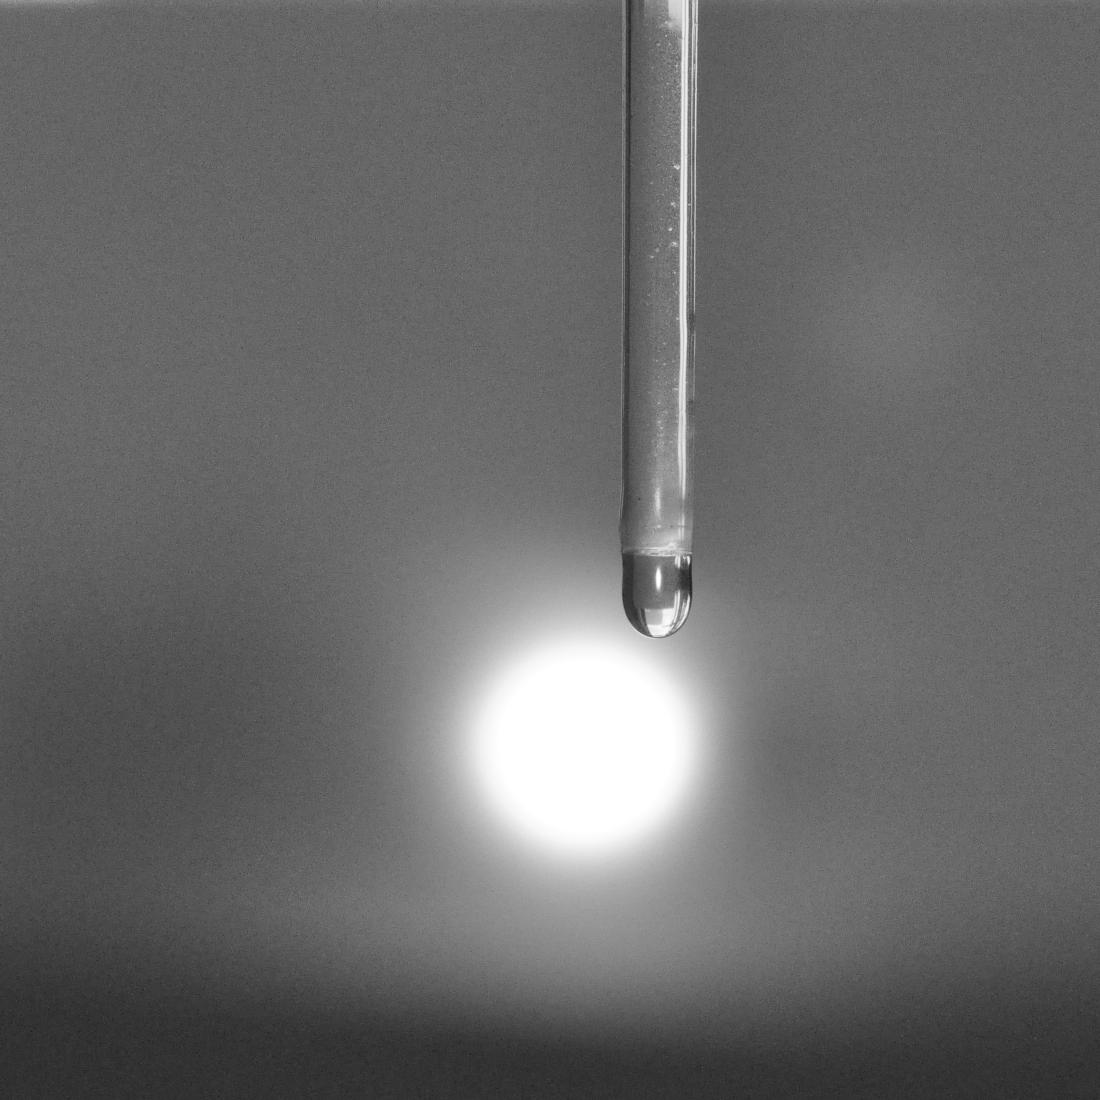
\includegraphics[height=0.4\textwidth]{photogoutte1}
}%
\parbox[l][0.4\textwidth][c]{0.35\textwidth}{
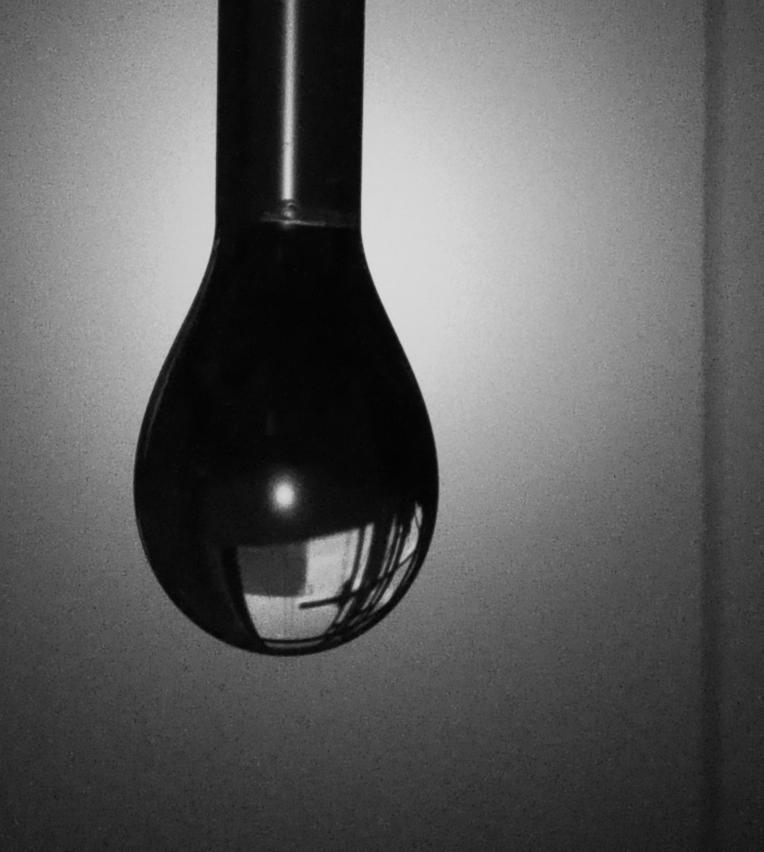
\includegraphics[height=0.2\textwidth]{photogoutte3}\hfill
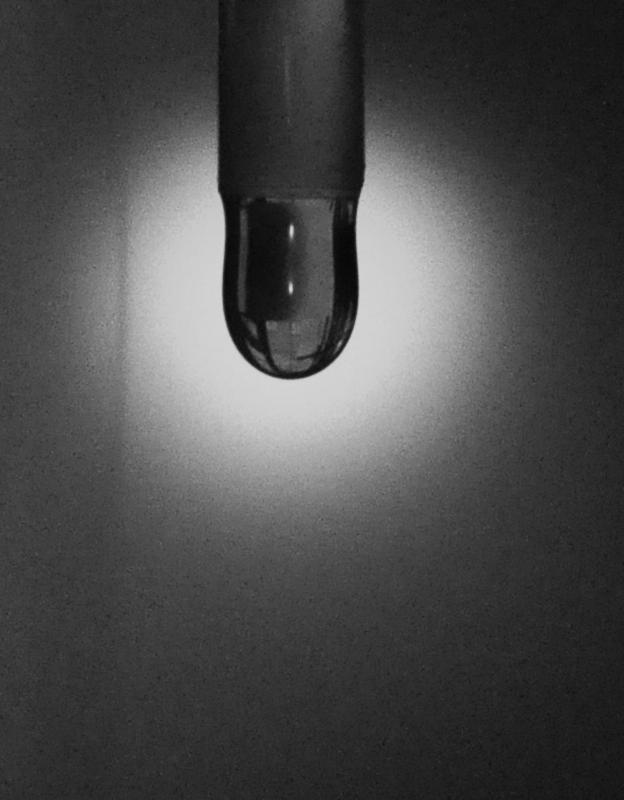
\includegraphics[height=0.2\textwidth]{photogoutte2}\\
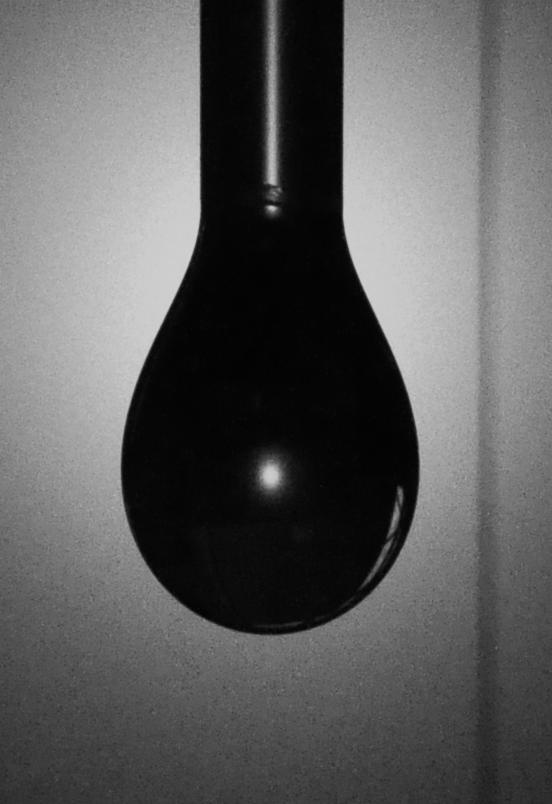
\includegraphics[height=0.2\textwidth]{photogoutte5}\hfill
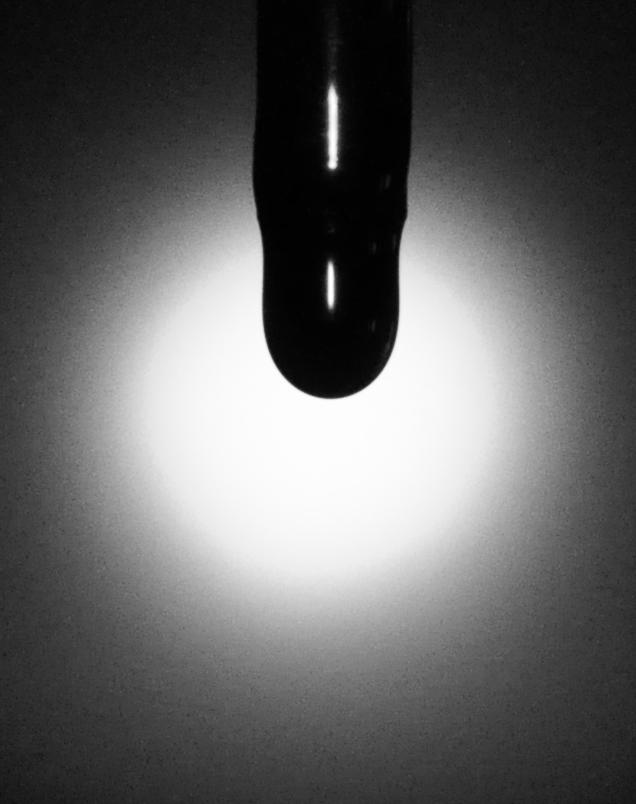
\includegraphics[height=0.2\textwidth]{photogoutte4}
}
\caption{\textbf{(left)} Experimental set-up for pendant drop surface
  tension measurement: a drop is hanging from a capillary tube
  (diameter here: $1.68\,$mm). A light source far behind the drop
  provides a bright background against which the drop is photographed.
  \textbf{(right, top row)} Drops of water and perfluorated oil close
  to the maximum volume before drop detachment. It is easy to see that
  the difference in surface tension has a tremendous effect on the
  drop shape. The pendant drop method consists in exploiting this
  strong dependency in order to determine an unknown surface tension.
  \textbf{(right, bottom row)} After optimising experimental
  conditions to get rid of spurious reflections and to enhance
  contrast.}
\label{fig:pendantdropphoto}
\end{figure}

\section*{Abstract}
\label{sec:abstract}

\begin{abstract}
  The pendant drop method for surface tension measurement consists in
  analysing the shape of a drop hanging from a capillary tube
  (Fig.~\ref{fig:pendantdropphoto}). The \gouttependante plug-in for
  \href{http://imagej.nih.gov/ij/}{ImageJ}~\cite{ImageJ} provides a
  tool to match a theoretical profile to the contour of a pendant
  drop, either interactively or automatically. The surface tension can
  then be easily calculated from the best matching parameters.
  Section~\ref{sec:description} describes the plug-in functionality,
  section~\ref{sec:prerequisites} lists the properties that the input
  image must have for the plug-in to give meaningful results. Sections
  \ref{sec:installation} and \ref{sec:usage} explain the installation
  and the usage of the plug-in. Finally sections~\ref{sec:theory} and
  \ref{sec:numerics} describe the underlying theoretical framework and
  the plugin's inner workings, respectively.
\end{abstract}


\section{Description}
\label{sec:description}

The pendant drop method is commonly used to measure surface tensions
of liquids. It consists in analysing the shape of a drop hanging
typically from a capillary tube and about to detach (sometimes the
inverse situation of a bubble forming at the bottom of a liquid is
preferred). The shape is very sensitive to the unknown interfacial
tension. The drop profile is described by only one non-dimensional
parameter (tip radius over capillary length), although in practice
five dimensional parameters can be adjusted within this plug-in: tip
position and curvature, tilt of symetry axis and capillary length. The
surface tension is calculated from the latter if the density
difference is given.

This plug-in allows interactive adjustment of a profile to an image of
a pendant drop. An estimate of the quality of the fit is logged to
ImageJ's log window. The plug-in can also be asked to improve the fit
by varying one or several of the parameters automatically (currently
by successive minimisation along chosen directions according to
Powell~\cite{Powell1965,Brandt1992}, see section~\ref{sec:numerics}).

This plug-in can also be used to estimate the surface tension from the
shape of a sessile drop.


\section{Prerequisites}
\label{sec:prerequisites}

The plug-in is run on a high contrast image of a pendant drop
(Fig.~\ref{fig:usage}-left). Pixel values are expected to be close to
zero within the drop, and close to saturation (i.e. 255 for 8-bit
images) outside. This is typically obtained by taking the picture of
the drop in front of a light background far away from the drop
(Fig.~\ref{fig:pendantdropphoto}). Bright spots well within the drop
are not a problem, but contrast should be good in the vicinity of the
contour. Avoid however thresholded (binary) black and white images,
which generally cause the minimisation algorithm to perform poorly. A
little bit of blurring on such images will improve the fitting
performance.

Draw a rectangular Region Of Interest (ROI) around the pendant drop
before calling the plug-in (Fig.~\ref{fig:usage}-middle). The ROI
should not include the inlet tube, but only the free surface of the
drop. A few ten or so pixels margin around the drop should be
sufficient. Including more of the outside region will not do harm, but
slow down calculations which take a time proportional to the area of
the ROI.


\section{Installing the plug-in}
\label{sec:installation}

As usual with ImageJ plug-ins, just put the jar into ImageJ's
\texttt{plugins} folder or a subfolder thereof. Restart ImageJ to see
the plug-in.


\section{Using the plug-in}
\label{sec:usage}

\begin{figure}
  \centering
  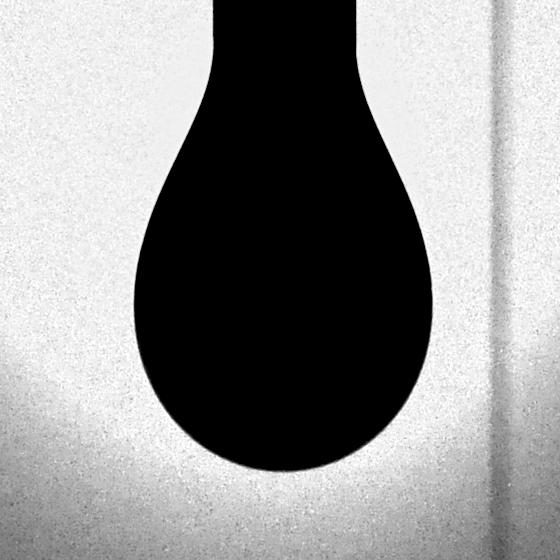
\includegraphics[width=0.25\textwidth]{eauContrasteMax}\hfill
  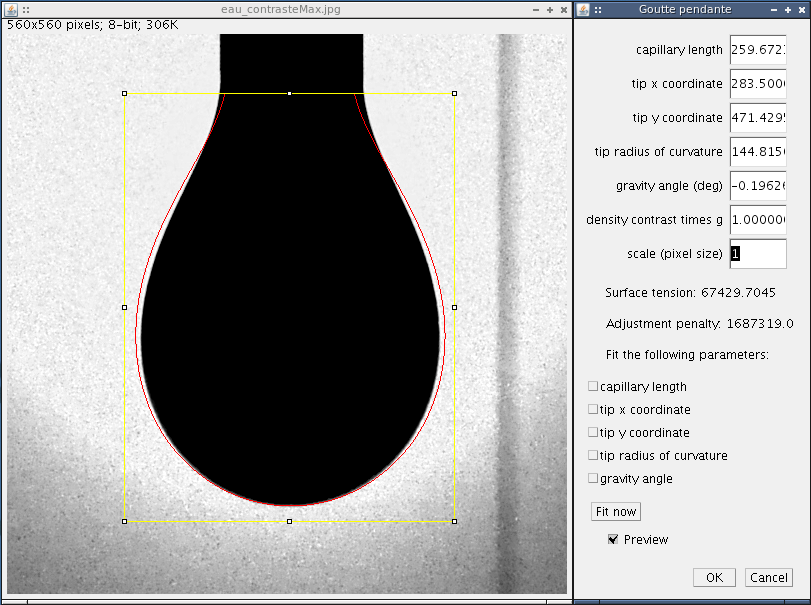
\includegraphics[width=0.36\textwidth]{eauContrasteMaxInitial.png}\hfill
  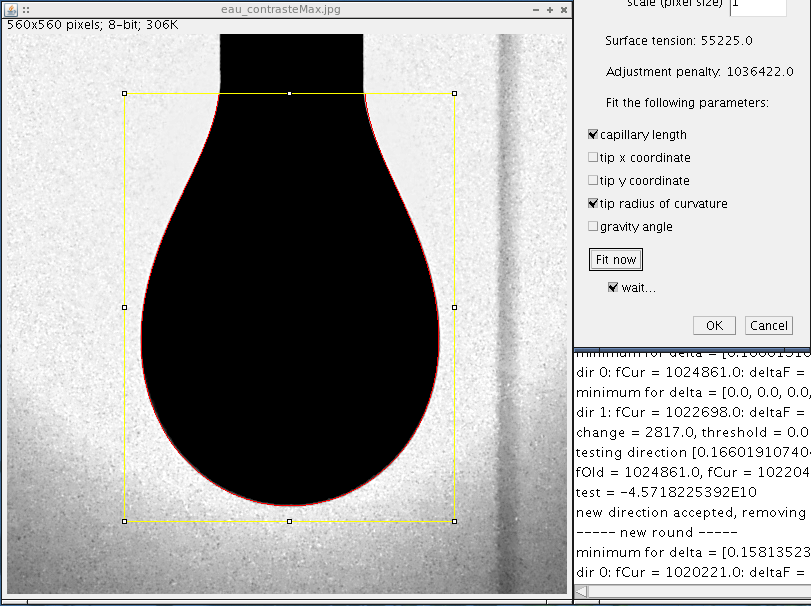
\includegraphics[width=0.36\textwidth]{eauContrasteMaxFit2.png}
  \caption{Plug-in usage. \textbf{(left)} starting image, high-pass
    filtered and contrasted just short of saturating black and white
    levels. \textbf{(middle)} image with rectangular ROI selection and
    initial guess next to plug-in dialog. \textbf{(right)} automatic
    ajustment under way. The progress and decrease of the penalty
    value is documented in the Log-window in the lower right.}
  \label{fig:usage}
\end{figure}

Fill in any parameter values you know, and check the plausibility of
the initial guess for the others. If the image was calibrated for
spatial scale, the corresponding scale is proposed by the plug-in (but
beware that ImageJ's dialogs round values to the number of digits
shown, so double-check in case your pixel size is much smaller than
unity) and all length scales are expressed in calibrated units. If the
image is not calibrated all lengths are given in pixels, including the
resulting capillary length.

Check the preview box so that the calculated profile is shown as an
overlay (Fig.~\ref{fig:usage}-middle).

a) modify the parameters so as to improve the visual accordance of
theoretical profile and image. The adjustment penalty value shown in
the dialog serves as a quantitative measure of the agreement: it
should be made as small as possible.

b) check those parameters that the plug-in may adjust and click on
\texttt{fit} for automatic minimisation (Fig.~\ref{fig:usage}-right).
Only the previously checked parameters are varied when trying to find
an optimal shape. The overlay is updated accordingly. Note that the
minimisation algorithm can get trapped in a local minimum, so try
starting from different initial values and check whether the resulting
profile looks satisfactory.

To interrupt fitting at any time click once more on the \texttt{fit}
button.

Exit the plug-in by clicking on either OK or Cancel.

\paragraph{How to get the surface tension}
If the image was scale-calibrated, and a sensible value was entered
for the `\texttt{density contrast times g}' parameter (the difference
of the densities in/outside the drop multiplied by your planet's
gravitational acceleration), then the surface tension is indicated
directly in the dialog. For example if the \texttt{pixel size} is in
millimetres, and the \texttt{density contrast times g} is in grams per
square second and square millimetre (e.g.\ around
$9.8\,\mathrm{g}/\mathrm{mm}^2\mathrm{s}^2$ for water in air on
earth), then the indicated surface tension is in
$\mathrm{g}/\mathrm{s}^2$ or milli-Newton per metre. Otherwise the
surface tension $\sigma$ has to be calculated by hand from the
indicated capillary length using the formula $\sigma = \Delta\!\rho g
\ell_c^2$.


\section{Physics of the pendant drop}
\label{sec:theory}

\textit{\small This section describes the physics behind the pendant drop method.\medskip}

Because of the density difference between the inner liquid and outer
gas phase, the pressure jump across the interface varies with height,
implying that the surface curvature must vary as well. Indeed, if the
lowest point of the drop is taken as origin for the height coordinate
$z$, the pressure inside the drop is $p_{\mathrm{in}}(z=0) -
\rho_{\mathrm{in}} g z$ at a distance $z$ above it, while it is
$p_{\mathrm{out}}(z=0) - \rho_{\mathrm{out}} g z$ outside. $g$ denotes
gravitational acceleration and $\rho_{\mathrm{in/out}}$ the densities
of the respective phases. Noting $\Delta\! p_0 = p_{\mathrm{in}}(z=0)
- p_{\mathrm{out}}(z=0)$ the pressure drop at the drop tip, and
$\Delta\!\rho = \rho_{\mathrm{in}} - \rho_{\mathrm{out}}$ the density
contrast, we have a pressure jump across the interface $\Delta\! p(z)
= \Delta\! p_0 - \Delta\!\rho g z$ at height $z$. Note that the value
of $\Delta\! p_0$ is unkown beforehand (it depends on the geometry of
our set-up and the drop volume).

\begin{figure}
  \begin{captionbeside}{Notations. The drop profile is assumed to be
      axisymetric, and is described by the two cylindrical coordinates
      $R(s)$ and $Z(s)$ as a function of the curvilinear parameter
      $s$. The local tilt $\psi$ with respect to the axis normal
      enters the expression for the interface curvature, and is
      related to $R$ through $R' = \cos\psi$. We have spherical
      symetry at the very tip, with radius $r_0$.}
\begin{tikzpicture}
  %\grid{3cm}{3cm}
  \pgftext{\pgfimage[height=15em]{dropsketch}}
  \pgftext[bottom,right,x=-10mm,y=-6mm] {$r_0$}
  \pgftext[right,x=-5mm,y=-13mm] {$Z$}
  \pgftext[bottom,x=3mm,y=-9mm] {$R$}
  \pgftext[bottom,left,x=18mm,y=-7mm] {$\psi$}
  \pgftext[x=-9mm,y=11mm] {$\rho_{\mathrm{in}}$}
  \pgftext[x=-20mm,y=11mm] {$\rho_{\mathrm{out}}$}
\end{tikzpicture}
\end{captionbeside}
\label{fig:notations}
\end{figure}

This pressure jump is due to surface curvature and surface tension
$\sigma$. It is related to the mean curvature $\bar\kappa$ by Laplace's
formula $\Delta\! p(z) = \sigma \bar\kappa(z)$.  We parametrise the drop
surface in cylindrical coordinates as $(R(s), Z(s))$, where $s$ is the
curvilinear distance to the tip. Expressing the mean curvature as a
function of $R$, $Z$ and the angle $\psi$ between the tangent plane to
the interface and the horizontal: $\ud R/\ud s = \cos\psi$, we obtain
the following expression for the pressure equilibrium:

\[\label{eq:shape}
  - \frac{1}{\ell_c^2} \sin\psi =
  \frac{\ud}{\ud s}\left( \frac{\ud\psi}{\ud s} + \frac{\sin\psi}{R} \right).
\]

 The boundary conditions at the drop tip are $\psi(0)=0$ and $\ud\psi
/ \ud s = p(0)/2\sigma = 1/r_0 = \mathrm{const.}$, where $r_0$ is the
radius of curvature of the drop tip which has locally spherical
symetry. Scaling all lengths by the characteristic length $\ell_c =
\sqrt{\sigma/\Delta\!\rho g}$ (called \emph{capillary length}) yields
one universal drop shape equation

\begin{equation}\label{eq:shapeNonDim}
  - \sin\psi =
  \frac{\ud}{\ud s}\left( \frac{\ud\psi}{\ud s} + \frac{\sin\psi}{R} \right)\\
  \mbox{with } \psi(0)=0 \mbox{ and } \psi'(0) = \ell_c/r_0,
\end{equation}

Note that the solutions (i.e. all possible drop shapes) are fully
determined by the choice of the initial condition for $\psi'(0)$,
which is just the ratio of the capillary length and the radius of
curvature of the drop tip.

\section{What the plug-in does internally}
\label{sec:numerics}

\minisec{numérical integration}
The equation~(\ref{eq:shapeNonDim}) is integrated for a given parameter
$\ell_c/r_0 = 1/r_*$ using a fourth order Runge-Kutta scheme. Near the
drop tip the integral equation becomes singular as $R\to 0$, but the
solution itself is perfectly regular: it is simply a nearly perfectly
spherical profile (at least at distances small with respect to
capillary length and tip radius). We can thus use an analytical
solution to get away from the singularity at $R=0$. The leading order
terms of that solution are

\[
\left.%
\begin{array}{lll}
R & = & r_*\sin\frac{s}{r_*} + \frac{s^5}{40 r_*^2} + O(s^6) \\
Z & = & \frac{1}{2r_*} s^2 (1 + (\frac{1}{16} - \frac{1}{12r_*^2}) s^2) + O(s^6)\\
\psi & = & s/r_* (1-s^2/8) + O(s^5)
\end{array}\right\}
\mathrm{for}\quad s \ll 1 \wedge s \ll r_*
\]

We use this solution to calculate the first piece of drop contour
where $s \ll 1$ and $s \ll r_*$. Then we continue through numerical
integration.

\minisec{estimate the qualitiy of the obtained solution}
The resulting drop contour is then rescaled, translated and rotated
according to the given parameters (tip position, curvature, \dots) and
overlayed as theoretical contour $\mathcal{C}$ on the drop image. An
adjustment penalty value is finally calculated as the sum over all
pixels in the Region Of Interest

\[
\mathcal{P} = \sum_{\mathrm{pixel}\ p \in \mathrm{ROI}} \mathrm{Err}(p)
\]

\noindent of per-pixel-penalties $\mathrm{Err}(p)$, which are
determined from the pixel intensity value $I(p)$ as

\[
\mathrm{Err}(p) = \left\{ \begin{array}{ll}
I(p) & \textrm{if } p \textrm{ is inside the drop contour } \mathcal{C} \\
I_{\mathrm{max}}-I(p) & 
\textrm{if } p \textrm{ is outside the drop contour } \mathcal{C}
\end{array} \right.
\]

The rationale behind this penalty function is to count drop and
non-drop pixels as penalty for the calculated contour if they are on
the wrong side. The input image is such that pixels belonging to the
drop on the image are near black, i.e. have a small, near zero intensity value: $I(p) \approx 0$. If they are within the calculated contour as they
should their $\mathrm{Err}(p)$ is small according to the formula
above, whereas they contribute a lot to the penalty if they are
outside~$\mathcal{C}$: $\mathrm{Err}(p) = I_{\mathrm{max}} - I(p)
\approx I_{\mathrm{max}}$ in this case. Likewise pixels outside the
drop belonging to the bright background on the image, near maximum
intensity $I_{\mathrm{max}}$, hardly contribute to the penalty
function if they are indeed outside the contour, but add their full
intensity value to $\mathcal{P}$ if they are inside~$\mathcal{C}$.

\minisec{optimize by varying parameters and iterating} In case
automated fitting of some parameters is requested, the plug-in tries
to minimise the penalty function by successively varying each free
parameter, searching for each the value that will yield the
best-fitting integrated drop contour. After all parameters have been
varied, the plug-in checks whether it is not more efficient to
minimise along another direction in parameter space, i.e.\ modify
several parameters concurrently, and possibly updates the list of
directions. The whole process is repeated until the change in the
penalty value after a full round becomes too small. For more details
see references~\cite{Powell1965,Brandt1992}.

\thebibliography{2}

\bibitem{ImageJ} W. S. Rasband, \textit{ImageJ}, U. S. National
  Institutes of Health, Bethesda, Maryland, USA,
  \url{http://imagej.nih.gov/ij/}, 1997-2010.
\bibitem{Powell1965} M. J. D. Powell, \textit{Computer Journal}
  \textbf{7} (1965) 155
\bibitem{Brandt1992} S. Brandt, \textit{Datenanalyse}, BI-Wiss.-Verlag
  (Mannheim, Leipzig, Wien, Zürich) 3rd edition, ISBN 3-411-03200-6
  (1992)
\end{document}
